\begin{figure}[!htbp]
\centering
\caption{Reduced Form Relationship Between Covid-19-related Outcomes and Population Density in 1500}
\centering
\label{fig:reduced-form-lpd}
  \subcaptionbox{GDP Growth Rates in 2020 \label{fig:reduced-gdp-lpd}}{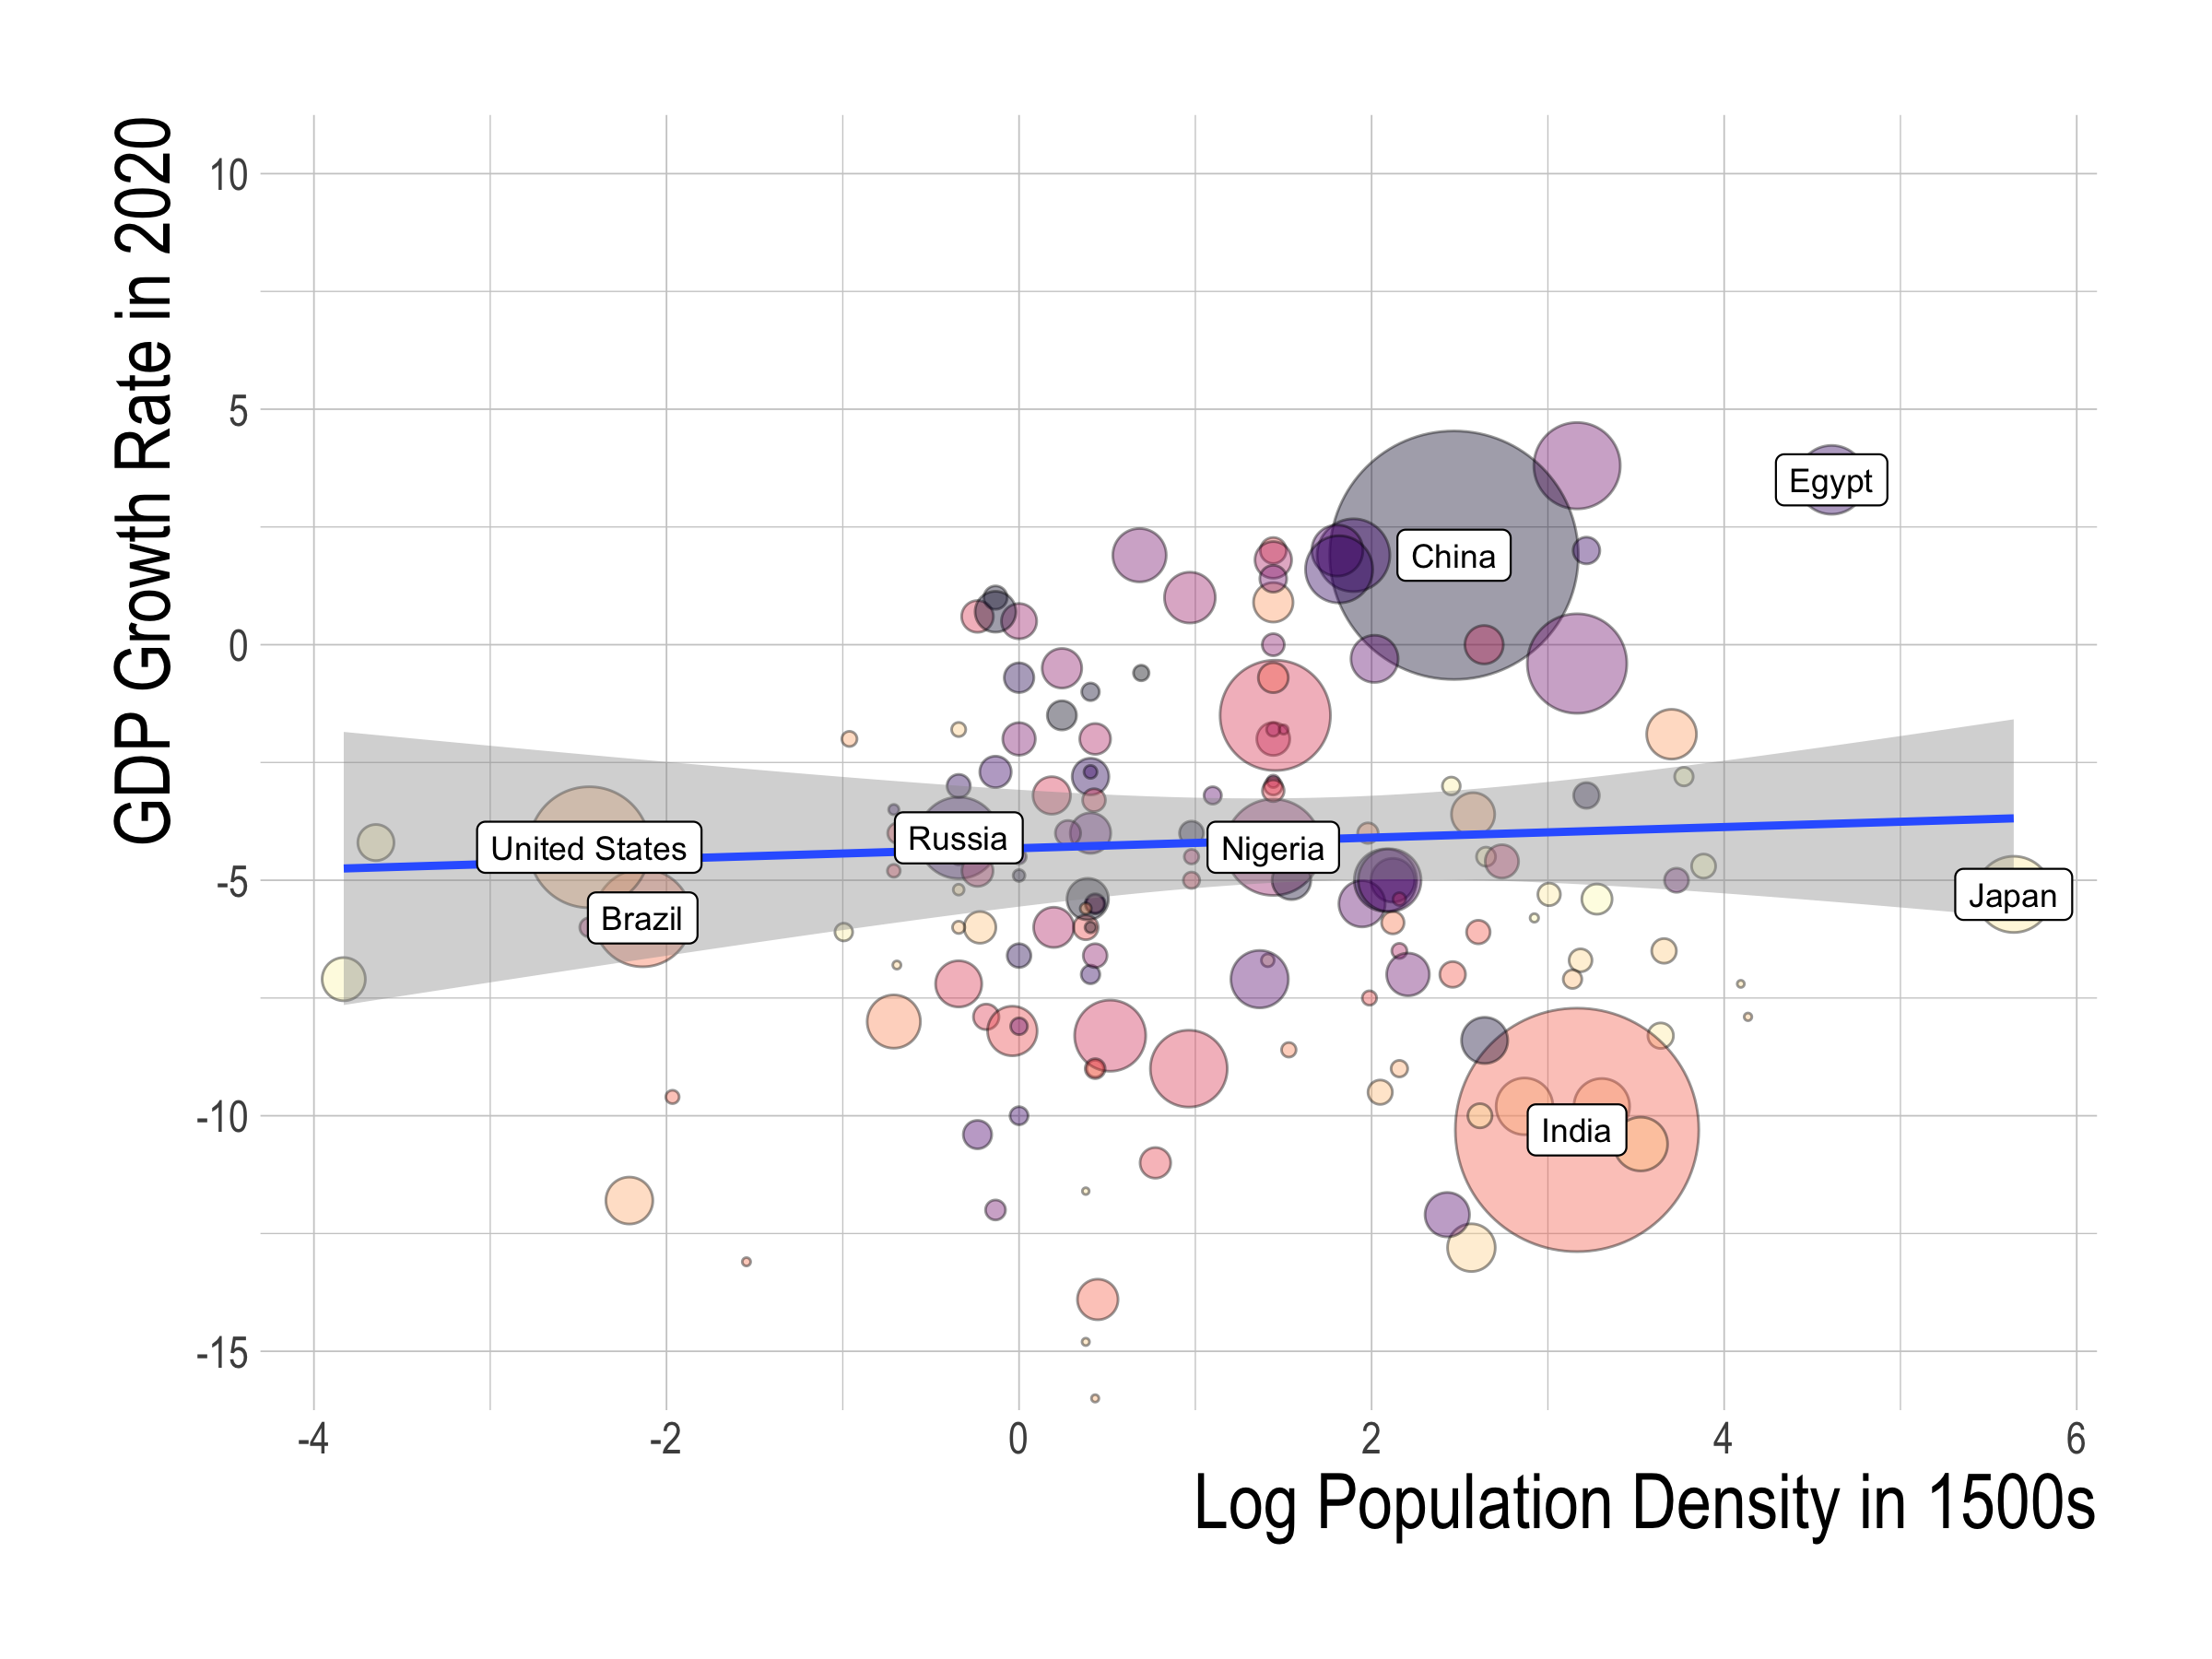
\includegraphics[width=5in]{plots/gdp_lpd1500s_noControls_popWeighted_ols.png}}
      \subcaptionbox{Total Covid-19-related Deaths Per Million\label{fig:reduced-deaths-lpd}}{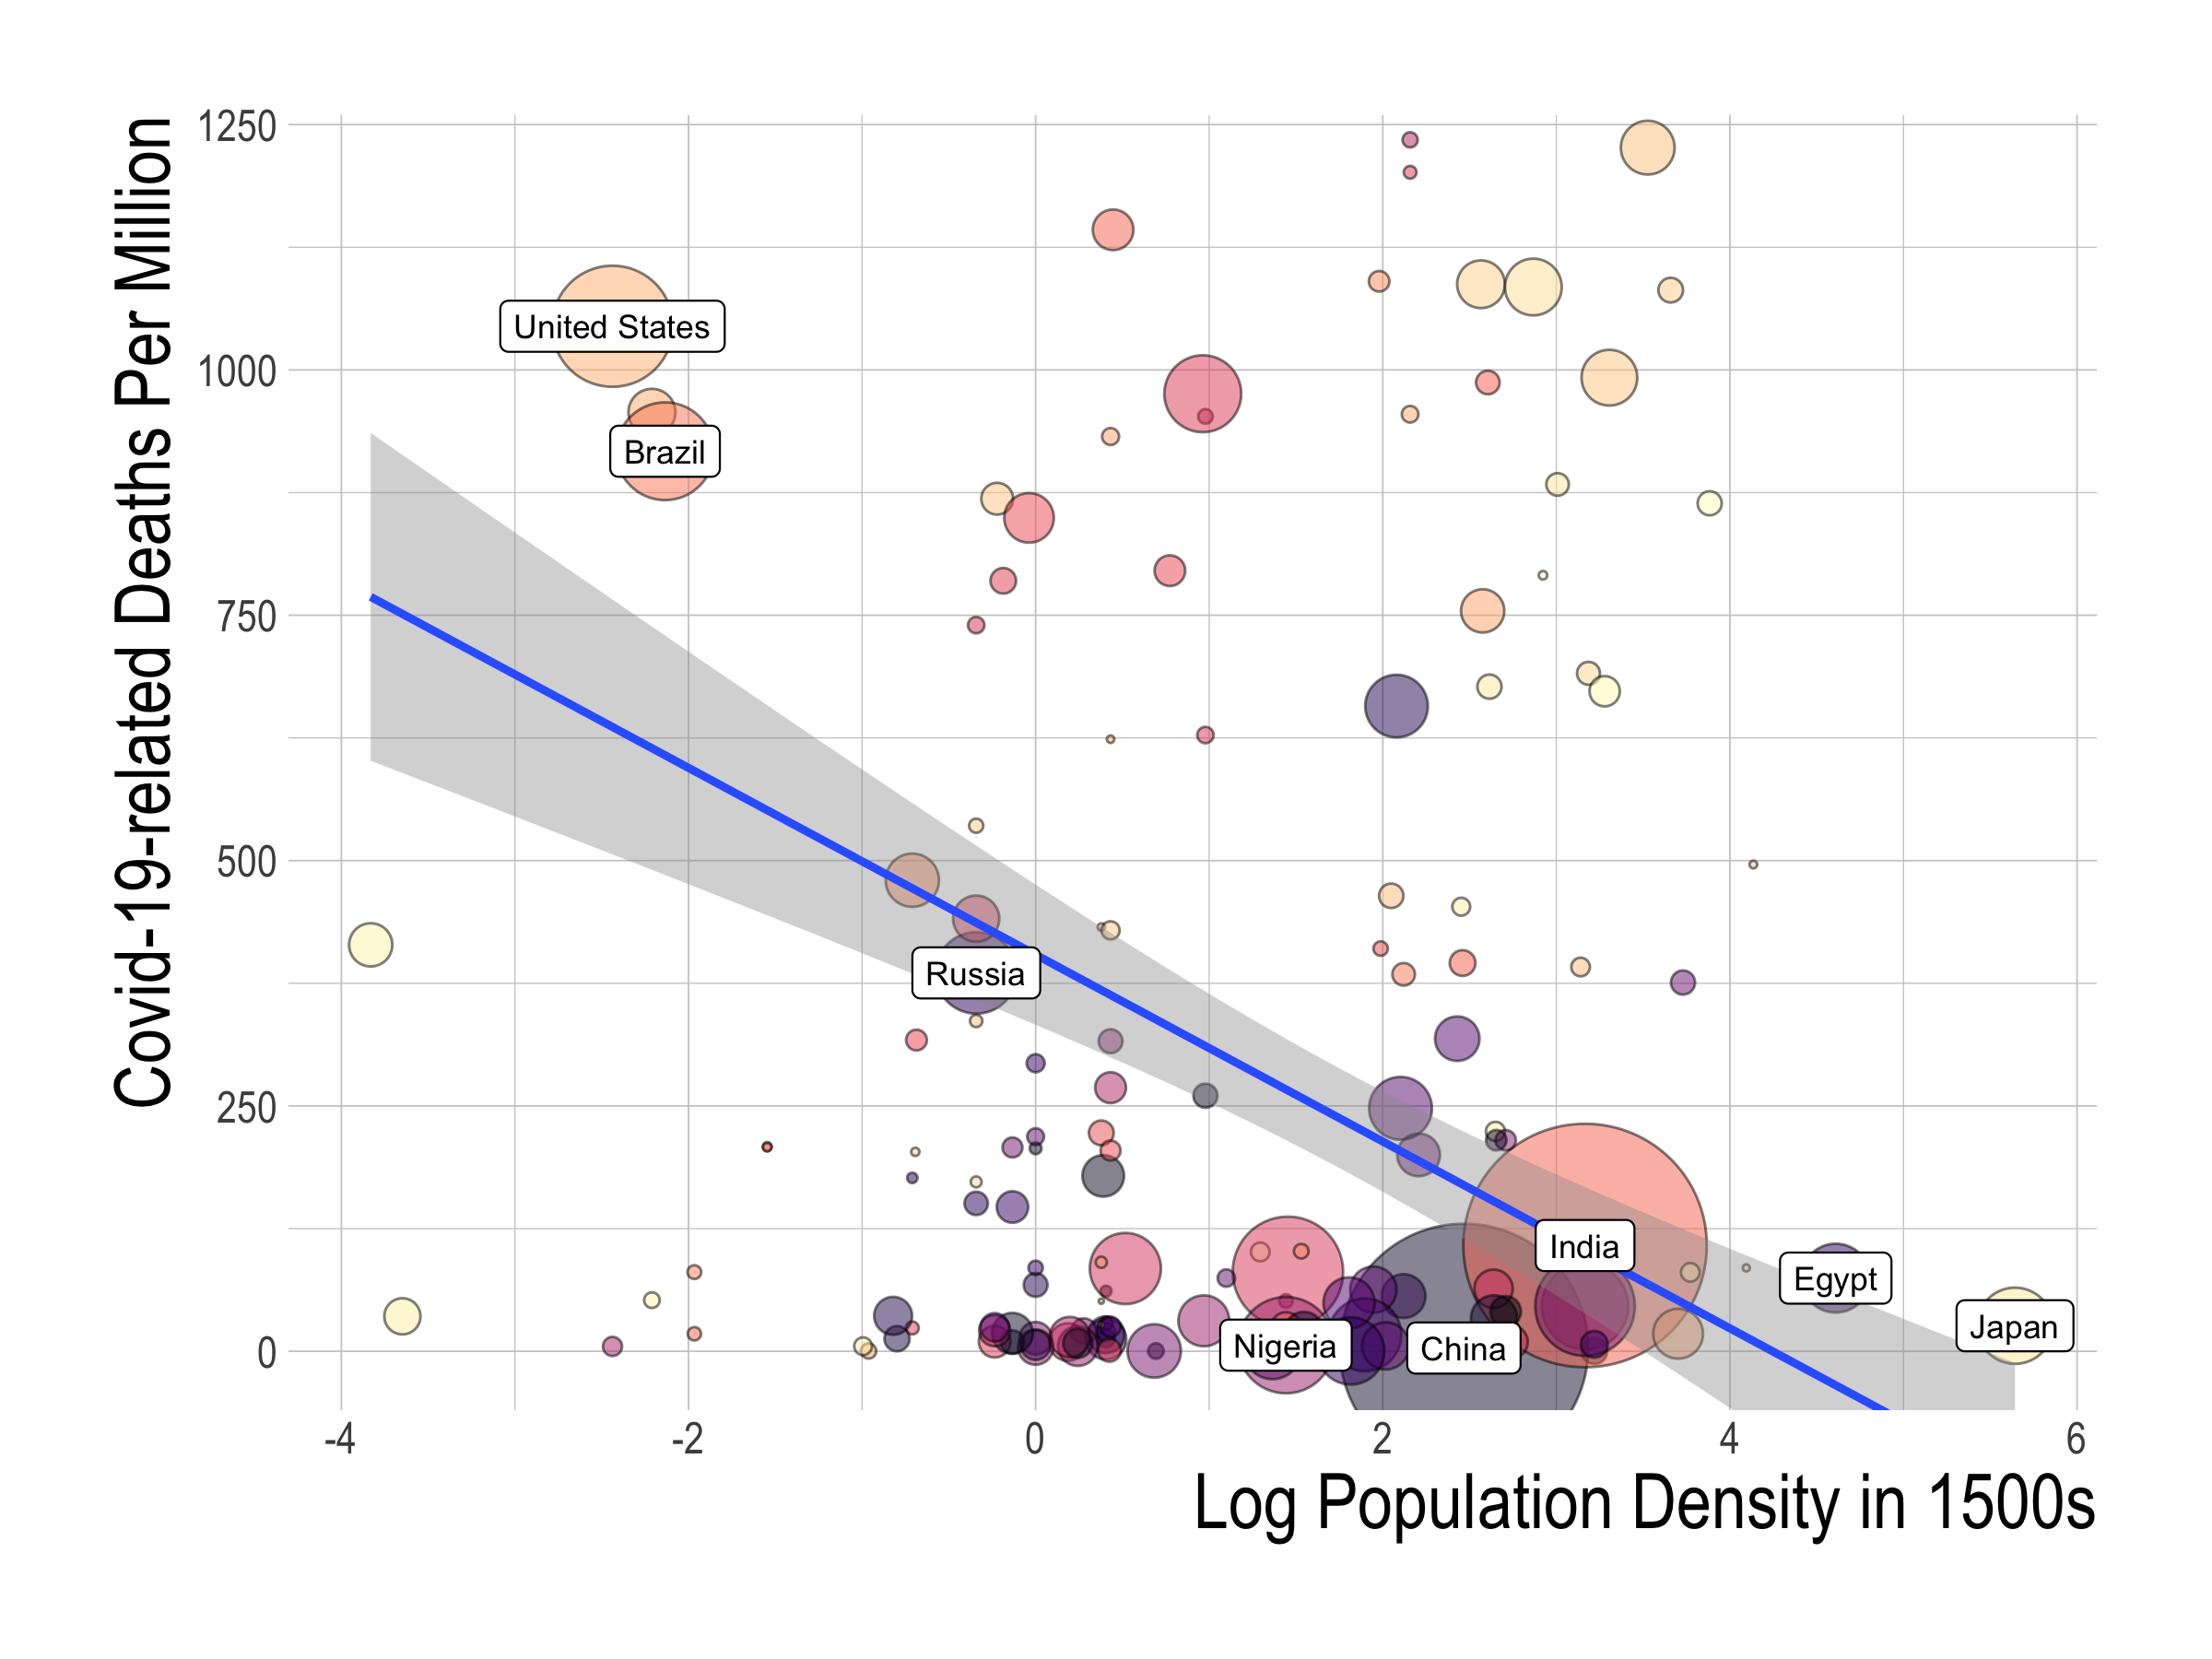
\includegraphics[width=5in]{plots/deaths_lpd1500s_noControls_popWeighted_ols.png}}
  \caption*{\textit{Notes:} The size of each observation point is proportional to the size of the population of each country. The colors vary depending on the level of the Democracy Index (Freedom House). The regression line corresponds to the reduced-form OLS regression without controls and weighted by population. The shaded area corresponds to the 95\% confidence interval.}
  
\end{figure}